\subsection{Introducción}
	Las máquinas de Turing son un dispositivo que permite idealmente resolver cualquier problema, debido a que tiene una memoria infinita, sin embargo está implementación no es posible de realizar y deben ser acotadas a una memoria o cinta finita, de tal forma que se dice que si una máquina de Turing es capaz de resolver un problema, este problema es computable (quiere decir que una computadora lo puede resolver). En caso contrario, se dice que el problema no es computable.\cite{LIBRO}
	
	
	De manera formal la máquina de Turing se define de la siguiente manera:

	\[ M=(Q, \Sigma, \Gamma, \delta, q_0, B, F) \]
	donde:
	\begin{description}
	 \item $Q$ es el conjunto finito de estados de la unidad de control.
	 \item $ \Sigma $ es el conjunto finito de símbolos de entrada
	 \item $ \Gamma $ es el conjunto completo de símbolos de cinta; $ \Sigma $ siempre es un subconjunto de $\Gamma$
	 \item $\delta$ Es la función de transición. Los argumentos de $\delta(q, X)$ son un estado $q$ y un símbolo de cinta $X$. El valor de $\delta(q, X)$, si está definido, es $(p, Y, D)$ donde:
	 \begin{enumerate}
	  \item $p$ es el siguiente estado de $Q$
	  \item $Y$ es el símbolo de $\Gamma$, que se escribe en la casilla que señala la cabeza y que sustituye a cualquier símbolo que se encontrara en ella.
	  \item $D$ es una dirección y puede ser $L$ o $ R$, lo que nos indica la dirección en que la cabeza se mueve, `izquierda` (L) o `derecha` (R), respectivamente
	 \end{enumerate}
	 \item $q_0$ es el estado inicial, un elemento de $Q$, en el que inicialmente se encuentra la unidad de control.
	 \item $B$ es el símbolo espacio en blanco. Este símbolo pertenece a $Gamma$ pero no a $Sigma$; es decir, no es un símbolo de entrada.
	 \item $F$ es el conjunto de los estados finales, un subconjunto de $Q$
	\end{description}

\subsection{Planteamiento de la práctica}
	El ejercicio a realizar en está actividad, es diseñar e implementar una máquina de Turing que duplique la cantidad de unos de una cadena ingresada, y que además, se muestre el procedimiento en una animación y se escriba en un archivo el historial de los pasos realizados por la máquina de Turing.
	
	
	Para la elaboración del programa, se realizó el siguiente diagrama que modela los estados y las transiciones que tiene la máquina.
	
	\begin{figure}[H]
		\begin{center}
			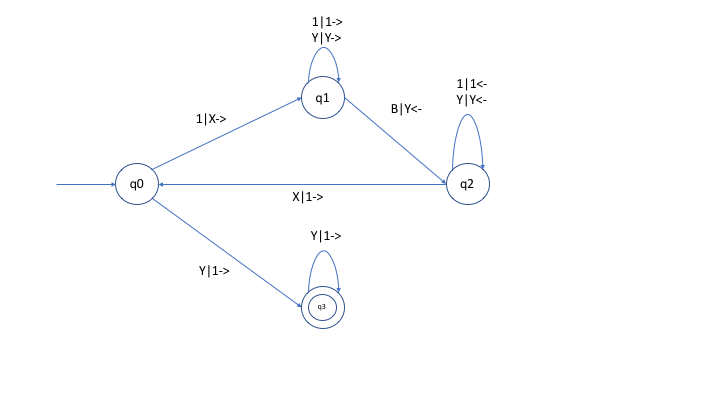
\includegraphics[scale=.5]{MT/img/maquina.png}
			\caption{Estados y transiciones usados}
			\label{fig:maquina}
		\end{center}
	\end{figure}
	